\chapter{Otimização Livre de Derivadas} \label{chap:3}


\section{Visão Geral}

\begin{itemize}


\item \textcolor{blue}{Motivate the use of derivative-free optimization.}
Frequentemente em problemas de engenharia os modelos utilizados são aproximações simplificadas da realidade, e em outros casos completamente desconhecidos.

Métodos de otimização sem derivadas são adequados em casos aonde o modelo matemático é não-explicito, custoso ou as derivadas não estão disponíveis, devido a inexistência do modelo explícito ou presença de ruídos impossibilitando a estimação das derivadas.

Os métodos de otimização sem derivadas procuram encontrar mínimos computando o menor número possível de pontos do problema, de modo a tentar minimizar também o tempo de execução da otimização.



\item \textcolor{blue}{Give a general presentation/introduction to derivative-free optimization}

\end{itemize}


%%%%
%%
\section{Método do Simplex de Nelder-Mead}

Também conhecido como Downhill Simplex Method, ou Amoeba Method, consiste em utilizar um poligono com n+1 vértices em n dimensões que se expande, contraí, ou reflete de modo a se mover em direção ao gradiente da função objetivo.

Um exemplo da execução do algoritmo de Nelder-Mead pode ser visto na figura~\ref{fig:neldermead}. A partir de um ponto inicial, o simplex se locomove como uma ameba até encontrar um ponto de mínimo.

\begin{figure}
\centering
\begin{subfigure}{.5\textwidth}
  \centering
  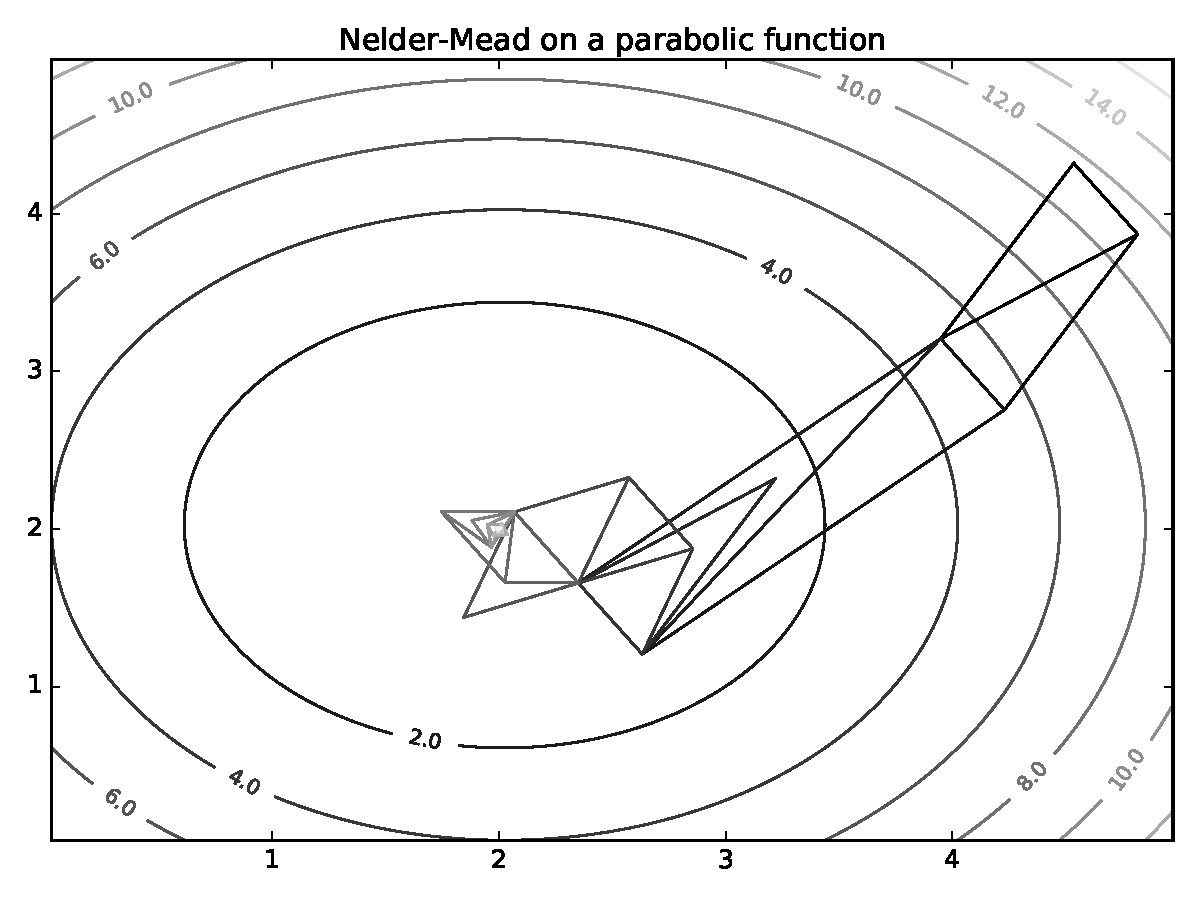
\includegraphics[width=\linewidth]{figs/neldermeadsimplex.pdf}
  \caption{Passos do Nelder-Mead}
  \label{fig:sub1}
\end{subfigure}%
\begin{subfigure}{.5\textwidth}
  \centering
  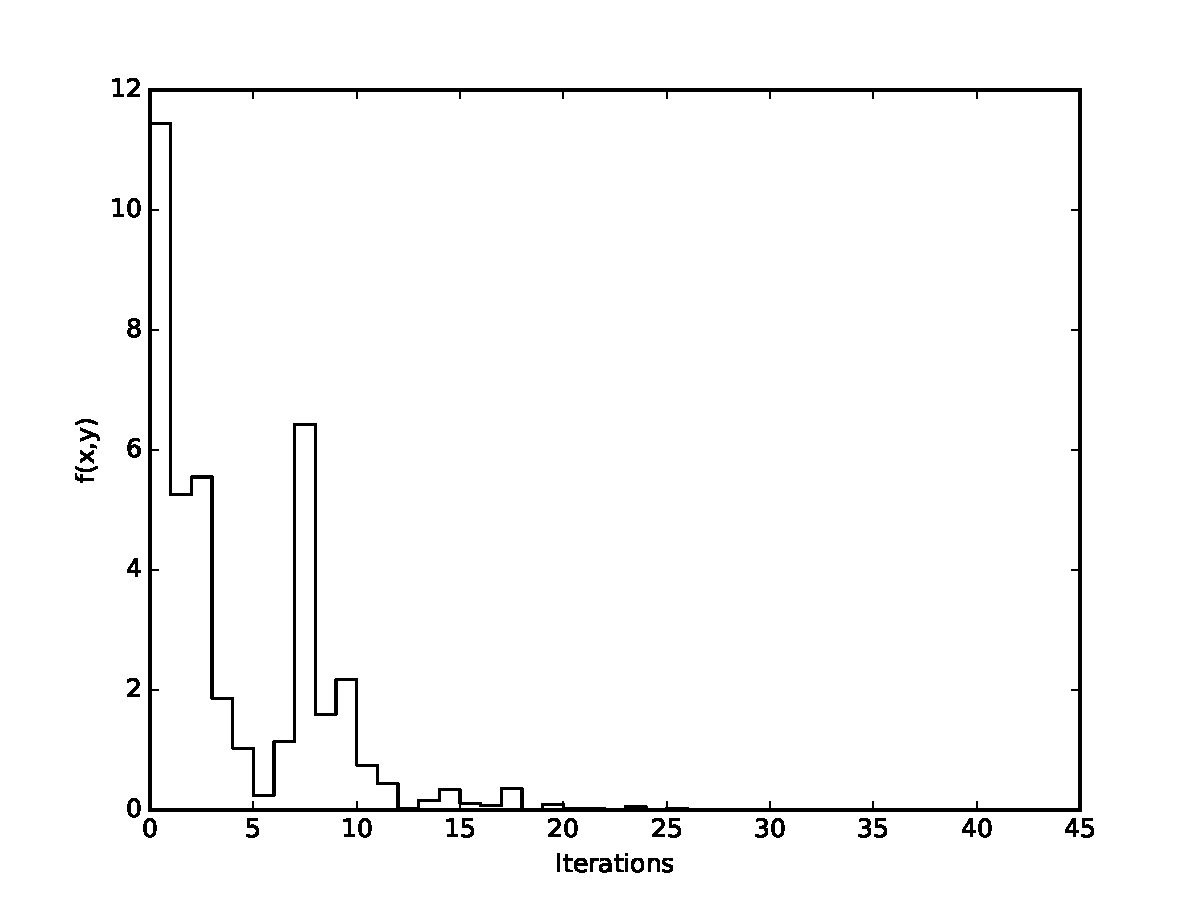
\includegraphics[width=\linewidth]{figs/neldermeadconvergence.pdf}
  \caption{Nelder-Mead aplicado em um parabolóide.}
  \label{fig:sub2}
\end{subfigure}
\caption{Demonstração do Nelder-Mead}
\label{fig:neldermead}
\end{figure}




\begin{algorithm}
    \caption{Nelder-Mead's Downhill Simplex}
    \label{alg:nm}
    \begin{algorithmic}[1] % The number tells where the line numbering should start
        \Require $X = (x_1, ... , x_{n+1})$ pontos de teste:
            \While{Não Convergiu}
                \State ordenar X; ($f(x _1) \leq f(({x} _2) \leq \cdots \leq f(x_{n+1})$) 
                \State Calcular o centroide $x_0$ de $(x_{1}, ... , x_{n+1})$
                \State Calcular $x_r$ refletido: $x_r = x_0 + \alpha(x_0 - x_{n+1})$ 
                
\BState \emph{(Reflecção)}                
                \If{  $f(f(x_1) < f(x_r) < f(x_n) $ }
                    \State $x_{n+1} \gets x_r$
                    \State Continue
                \EndIf

\BState \emph{(Expansão)}
                \If{  $f(f(x_r) < f(x_1)$ }
                    \State Calcular ponto expandido $x_e = x_0 + \gamma(x_r - x_0) $
                    \If{$f(x_e) < f(x_r)$}
                        \State $x_n \gets x_e$
                    \Else
                        \State $x_n \gets x_r$                  
                    \EndIf
                    \State Continue
                \EndIf
\BState \emph{(Contração)}
                \State Computar o ponto contraído $x_c = x_0 + \rho(x_{n+1} - x_0)$
                \If{$f(x_c) < f(x_{n+1})$}
                    \State $x_{n+1} \gets x_c$
                    \State Continue             
                \EndIf
\BState \emph{(Encolhimento)}
                \State $x_i \gets x_1 + \sigma(x_i - x_1), i=2 \dots n+1$
            \EndWhile
    \end{algorithmic}
\end{algorithm}



%%%
%%
\section{OrthoMADS}

Os métodos MADS (Mesh Adaptative Direct Search) são uma classe de métodos baseados ...


A cada iteração $ k $ são executados dois passos de busca, Search e Poll, analisando a feasibility e valor da função. O objetivo de cada nova iteração é encontrar um ponto $f(x) < f(x_k)$, aonde $x_k$ é o melhor ponto encontrado até a iteração atual. 

As buscas são feitas sempre em uma grade, definida por:

$M_k = \{x + \Delta^m_kDz : x \in V_k, z \in \mathbb{N}^{nD} \} \subset \mathbb{R}^n$
Aonde $M_k$ é o conjunto de pontos da grade, $x$ é o ponto mínimo atual, $\Delta^m_k$ é o parametro de tamanho da malha, $D$ é uma matrix $\mathbb{R}^{n \times n_D}$ composta por $n_D$ direções que definem um conjunto gerador position no $\mathbb{R}^n$. Para o OrthoMads e LtMads, D é simplesmente definida como $[I_n -I_n]$ aonde $I_n$ é a matriz identidade de dimensões $n$.

O passo search pode ser qualquer tipo de heurística que escolha um ponto mais adequado da malha para tentar acelerar a convergência.

O passo poll é a parte mais importante do método, que garante sua convergência. A cada iteração $k$ os pontos a serem utilizados são definidos por:

\begin{center}
$P_k = \{ x_k + \Delta^p_kd : d \in D_k\} \subset M_k$
\end{center}

Aonde  $x_k$ é o ponto atual e cada coluna de $D_k$ é formada por combinações inteiras das colunas de $D$ de forma a criar um conjunto gerador positivo. $\Delta^p_k$ é o \textit{parametro de tamanho de poll}.

Ambos LtMads e OrthoMads utilizam um parametro $\ell_k$ chamado de \textit{indíce de malha} para atualizar os parametros de tamanho de poll e search de acordo com esta lógica:


\begin{equation} \label{eq:meshsizeupdate}
\Delta^p_k = 2^{-\ell k} \text{ e }  \Delta^m_k = min\{1, 4^{-\ell_k}\}
\end{equation}

A cada nova iteração, se em uma iteração um novo \textit{incumbente} não é encontrado, ela é dita mal sucedida, e $\ell_{k+1} \gets \ell_k +1$ (reduzindo $\Delta^m_k$ e $\Delta^p_k$), por outro lado, se for encontrado um novo \textit{incumbente}, a iteração é dita bem sucedidade, e $\ell_{k+1} \gets \ell_k -1$ (aumentando $\Delta^m_k$ e $\Delta^p_k$). Devido a \ref{eq:meshsizeupdate}, no caso de uma iteração mal-sucedida o parametro de poll diminui mais rápido que o de malha, de modo a permitir o uso de muitos mais pontos, refinando a malha.


A diferença entre o OrthoMads e LtMads se dá na geração da base $D_k$. O LtMads utiliza uma matriz triangular inferior para a geração da base, fazendo permutações entre os elementos e completando ela em uma base maximal ou minimal, sem garantir ortogonalidade entre as direções, de modo que os ângulos entre as direções podem ser grandes, causando grandes cones de espaço não explorado.
Já o OrthoMads utiliza uma base maximal definida por $[H_k -H_k]$, aonde as colunas de $H_k$ formam um base ortogonal de $\mathbb{R}^n$. Além disso, os as direções de $D_k$ são inteiras, de modo que os pontos gerados estão automaticamente contidos na malha definida por $D=[I_n -I_n]$.

Para a geração de $D_k$, o OrthoMads utiliza a sequencia pseudo-aleatoria de Halton, que cobre mais uniformemente o espaço que uma sequência aleatória real, para  gerar vetores $u_t$.

A saída da sequência de Halton, no entanto, não respeita as restrições impostas pela malha. É necessário arrondar, escalar, e rotacionar o vetor $u_t$. O indíce $\ell$ é utilizado para transformar a direção $u_t$ na \textit{direção ajustada de Halton} $q_{t,\ell} \in \mathbb{Z}^n$, uma direção cuja norma é próxima a a $2^{\frac{|\ell|}{2}}$

HERE, BLACK MAGIC IS USED TO MAKE THE VECTOR ALIGN TO THE MESH.

Para definir $q_{t,\ell}$, primeiramente são definidas duas funções baseadas na t-ésima direção de Halton $u_t$:

$q_t(\alpha) = \text{round} \left ( \alpha \cfrac{2u_t - e}{||2u_t - e||} \right ) \in \mathbb{Z}^n \cap \left [ -\alpha - \cfrac{1}{2}, \alpha + \cfrac{1}{2}  \right ]^n$

Aonde \textit{round} é a operação arrendodar para cima ($round(0,5)=1$, $round(-0,5) = -1$) e $\alpha \in \mathbb{R}_+$ é um fator de escala. 

Desta forma, temos um problema de otimização, precisamos encontrar um $\alpha_{t,\ell}$ tal que $||q_t(\alpha_{t,\ell})$ seja o mais próximo possível de $2^{\frac{|\ell|}{2}}$ sem ultrapassá-lo.

\begin{align*}
\alpha_{t,\ell} \in \underset{\alpha in \mathbb{R}_+}{\textit{argmax}} & ||q_t(\alpha)|| \\
\text{s.t.} & ||q_t(\alpha)|| \leq 2^{\frac{|\ell|}{2}}
\end{align*}

O problema pode ser resolvido facilmente, já que que os degraus da função $||q_t(\alpha)||$ acontecem em todos os $\alpha$ no conjunto

\begin{center}
$ \left \{ \cfrac{(2j+1)||2u_t - e||}{2|u^i_t - e|} : i = 1,2,\dots,n,j \in \mathbb{N} \right \}$
\end{center}
De forma que o problema pode ser solucionado varrendo os pontos do conjunto.

Com um vetor normalizado e na malha, $q \in \mathbb{Z}^n$, é necessário transformá-lo em uma base ortonormal de $\mathbb{R}^n$. Para isto é utilizada a transformação de Householder:

\begin{equation}
H = ||q^2||(I_n - 2vv^T),\textit{ onde }v = \cfrac{q}{||q||}
\end{equation}

Aonde $H$ é uma base ortonormal gerada a partir de $q$.

Com a base ortonormal criada, podemos utilizar o algoritmo~\ref{alg:orthomads}, comum ao LtMads e OrthoMads.

ALGO MAIS DEVE SER ESCRITO AQUI, MAS OQ?


\begin{algorithm}
    \caption{OrthoMads}
    \label{alg:orthomads}
    \begin{algorithmic}[1] % The number tells where the line numbering should start
\BState \emph{[0] Inicialização}   
                \State $x_0 \in \Omega , \ell_0 \gets 0, k \gets 0, t_0 \gets p_n$ 
            \While{Não Convergiu}
\BState \emph{(ITERAÇÃO $k$)}                
            \State Search (opcional)
			\State Avalia $ f $ em um conjunto finito $S_k \subset M_k $
\State \emph{POLL}
    \If{o tamanho do parametro POLL é o menor até então ($ \Delta^p_k = \text{min} \{ \Delta^p_j : j=  0,1,\dots,k \}$)} 
    \State $t_k \gets \ell_k + t_0$
    \Else{ (Já foram considerados tamanhos menores)}
    \State $t_k \gets 1 + \text{max} \{t_j:j=0,1,\dots,k-1\}$
    \EndIf
    \State Computa $ u_{tk} , q_{tk}   \ell_k $ and $ D_k = \big[ H_{tk} \text{    } -H_{tk} \big] $
\BState \emph{UPDATES}                
	\If{ A iteração foi bem sucedida ( se existe um $x_s \in S_k \text{ ou } x_p \in P_k$ tal que $f(x_s) < f(x_k)$ ou $ f(x_p) < f(x_k)$ }
		\State $x_{k+1} \gets x_s $ or $x_p$
		\State $\ell_{k+1} \gets \ell_k - 1$
	\Else {(iteração falhou)}
		\State $x_{k+1} \gets x_k$
		\State $\ell_{k+1} \gets \ell_k + 1$
    \EndIf
    \State $k \gets k + 1$
    \EndWhile
    \end{algorithmic}
\end{algorithm}



%%%%%%%%%%%%%%%%%
